\documentclass[conference]{IEEEtran}
\IEEEoverridecommandlockouts
\usepackage{cite}
\usepackage{amsmath,amssymb,amsfonts}
\usepackage{graphicx}
\usepackage{textcomp}
\usepackage{xcolor}
\usepackage{booktabs}
\usepackage{multirow}
\usepackage{url}
\usepackage{microtype}
\usepackage{tikz}
\usetikzlibrary{positioning,arrows.meta,fit,backgrounds,matrix}
\usepackage{listings}
\lstset{
  basicstyle=\ttfamily\scriptsize,
  breaklines=true,
  frame=single,
  frameround=tttt,
  belowskip=0pt,
  aboveskip=4pt
}

\newcommand\Logan[1]{\leavevmode{\footnotesize\textbf{[Logan: #1]}}}
\newcommand\Alex[1]{\leavevmode{\footnotesize\textbf{[Alex: #1]}}}
\newcommand\Joe[1]{\leavevmode{\footnotesize\textbf{[Joe: #1]}}}
\newcommand\Kellan[1]{\leavevmode{\footnotesize\textbf{[Kellan: #1]}}}


\begin{document}

\title{SensorWF: A FAIR Generalizable Workflow Framework\\for Multi-Domain Scientific Time-Series Analysis}

\author{
  \IEEEauthorblockN{Author Name\textsuperscript{1},
                    Author Name\textsuperscript{2}}
  \IEEEauthorblockA{\textsuperscript{1}\textit{Department, Institution, City, Country}\\
                    \textsuperscript{2}\textit{Department, Institution, City, Country}\\
                    email@example.com}
}

\maketitle

\begin{abstract}
Scientific sensor data pervades disciplines from spacecraft engineering and clinical medicine to atmospheric science---and in each case, the analytical pipeline follows the same skeleton: ingest raw archives, assess quality, engineer features, annotate semantically, and record provenance. Yet these pipelines are routinely published as monolithic, domain-specific scripts whose assumptions remain implicit and whose components resist reuse across disciplinary boundaries. We present \textbf{SensorWF}, a FAIR-annotated workflow framework for generalizable scientific time-series analysis. A five-module reusable core (M1--M5) with typed I/O contracts forms the analytical backbone; a \emph{domain adapter} pattern confines all domain-specific logic to M1 so that M2--M5 execute identically across disciplines, encoding domain assumptions in a machine-readable component registry so that any sensor domain can be integrated and reused without altering the analytical core. Domain-specific analyses attach as \emph{use-case extensions} without modifying the core. Runtime PROV-O/ProvONE provenance traces---including SHA-256 checksums for all file-path entities---and SSN/SOSA-aligned OWL ontologies are emitted as first-class outputs. To validate generalizability, we instantiate SensorWF across three scientifically distinct domains---spacecraft telemetry, ambulatory ECG, and atmospheric climate---and demonstrate synthetic fault injection and multi-detector anomaly detection as a representative use-case extension. Results confirm that a single codebase, parameterised solely through M1 adapters of approximately 150 lines each, supports complete analytical pipelines across domains with markedly different sampling rates, channel counts, and fault taxonomies. All code, component registry, ontology artefacts, and datasets are released as an open scientific object.
\end{abstract}

\begin{IEEEkeywords}
computational workflows, FAIR principles, domain adaptation, sensor analytics, anomaly detection, PROV-O, ProvONE, knowledge graph, reproducibility
\end{IEEEkeywords}

%% =========================================================
\section{Introduction}
%% =========================================================

Sensor-driven scientific disciplines share a computational burden that receives little formal architectural attention. Raw measurements must be ingested, corrected for artefacts, and transformed into analysis-ready feature representations---each stage encoding domain assumptions about sampling rates, quality thresholds, and channel semantics that are seldom made explicit or machine-readable. Downstream analyses then layer further domain-specific logic on top of this shared skeleton.

Despite this structural commonality, pipelines across domains are almost universally developed in isolation as monolithic, domain-specific scripts. The resulting fragmentation prevents reuse, makes cross-domain comparisons unreliable, and renders post-publication audit practically impossible. The eScience and open-science communities have called for pipelines to be treated as first-class scientific objects whose provenance can be traced, shared, and reused \cite{wilkinson2016fair,garijo2022fair}.

This paper presents \textbf{SensorWF} (\emph{Generalizable FAIR Sensor Analytics Workflow}), a framework for multi-domain scientific sensor time-series analysis. The five-module core handles ingestion (M1), quality assessment (M2), feature engineering (M3), semantic annotation (M4), and provenance export (M5). Domain-specific analysis tasks attach as \emph{use-case extensions}: we demonstrate synthetic fault injection (E1) and automated anomaly detection (E2). Fig.~\ref{fig:architecture} illustrates the full architecture.

\subsection{Contributions}
Our contributions include:
\begin{enumerate}
  \item \textbf{A generalizable five-module workflow core} (M1--M5) with typed I/O contracts and explicit scientific assumptions. The \emph{domain adapter} pattern isolates domain-specificity in M1; M2--M5 execute identically across disciplines via adapter-supplied configuration.
  \item \textbf{A machine-readable component registry} (\texttt{components.json}) encoding domain assumptions as typed ports, configuration parameters, domain tags, and ProvONE URIs for every module---so that any sensor domain can be integrated and reused without altering the analytical core---enabling automated composition, discovery, and extension.
  \item \textbf{Runtime provenance and semantic annotation.} SensorWF emits PROV-O/ProvONE Turtle provenance for every execution---including SHA-256 checksums for all file-path entities---and maps analytical evidence to domain OWL ontologies (SSN/SOSA-aligned \cite{haller2019ssn,compton2012ssn}), producing SPARQL-queryable knowledge graphs.
  \item \textbf{Cross-domain evaluation via an anomaly detection use case.} We demonstrate SensorWF across three well-established datasets using E1 fault injection and E2 multi-detector evaluation as a concrete analytical extension.
\end{enumerate}

%% =========================================================
\section{Background and Related Work}
\label{sec:background}
%% =========================================================

\subsection{FAIR Computational Workflows}

The FAIR principles, being Findable, Accessible, Interoperable, and Reusable, were developed by Wilkinson et al. for a persistent issue in scientific publishing, in which data and software are routinely produced but are effectively lost to the community due to a lack of metadata, open licenses, and standard formats needed for reuse \cite{wilkinson2016fair}. When applied to computational workflows, the FAIR framework requires pipelines to include machine-readable metadata, typed I/O specifications, and explicit documentation of assumptions, enabling other researchers to discover, cite, and extend workflows without examining source code \cite{garijo2022fair}. Gustafsson et al. describe WorkflowHub, a registry for computational workflows that supports FAIR sharing and scholarly attribution via RO-Crate packaging and open standards including CWL and the GA4GH TRS API \cite{gustafsson2025workflowhub}. WorkflowHub is intended to enable the discovery and reuse of workflows in an accessible and interoperable manner. This goal is achieved through the adoption of open standards and tools, including CWL, RO-Crate, Bioschemas, and the GA4GH TRS API, in alignment with the FAIR principles. Our work, SensorWF, advances this ecosystem by explicitly encoding domain assumptions in a machine-readable component registry, allowing any sensor domain to be integrated and reused without altering the analytical core.
\Alex{Make sure this is in the paper: ``\colorbox{yellow}{encoding domain assumptions} in a machine-readable component registry, allowing any sensor domain to be integrated and reused without altering the analytical core''}

\subsection{Scientific Provenance}

In scientific research, provenance refers to the comprehensive documentation of how a result is generated. This record encompasses the input data, applied transformations, software versions, and the timing of each procedural step. In the absence of such documentation, published results cannot be independently verified, and subsequent analyses lack the means to assess the reliability of their inputs. The W3C PROV Ontology (PROV-O) serves as the international standard for representing provenance in a machine-readable format \cite{provo2013}. It models computations as graphs that connect data artifacts, processing activities, and responsible agents through standardized relationships. These graphs are programmatically queryable, ensuring that execution histories remain accessible for inspection even after the original researcher is no longer involved. ProvONE \cite{missier2013provone} extends PROV-O for scientific workflow systems by introducing constructs for pipeline programs, their input and output ports, and individual executions, which aligns well with modular frameworks. In practice, PROV-O has been implemented in different domains, for example, to enhance audit trails in epidemiological pipelines \cite{mitchell2022fair} and integration into Earth Observation processing platforms \cite{omidi2025openeo}, among others.

\subsection{Ontologies, Vocabularies, and Knowledge Graphs}

Ontologies, controlled vocabularies, and knowledge graphs establish a semantic foundation for representing scientific data in a consistent and machine-interpretable manner \cite{wilkinson2016fair}. This foundation is particularly critical in sensor-based workflows, where raw channel names and derived features are often highly domain- or dataset-specific and may lack sufficient meaning outside the original data-collection context. For example, a telemetry voltage channel, an ECG signal lead, and an atmospheric temperature measurement may all be represented numerically as time-series observations, yet they correspond to distinct instruments and physical systems. In the absence of formal semantic descriptions, these meanings remain embedded in code, documentation, or researcher knowledge, thereby restricting the reusability and transferability of workflows across domains.

Sensor-oriented vocabularies such as SSN and SOSA address this issue by providing standardized concepts for describing sensors, observations, platforms, and related entities \cite{haller2019ssn}. These vocabularies allow sensor datasets to be represented using a shared conceptual structure while still permitting domain-specific extensions through ontologies. In this way, a workflow can preserve the specialized meaning of each domain, such as spacecraft subsystems or biomedical signal classes, while maintaining interoperability with broader semantic web standards.

Knowledge graphs implement these semantic models by representing entities and relationships as interconnected graph structures. In scientific time-series workflows, a knowledge graph can link engineered features to their source channels, relevant domain concepts, and supporting evidence. This structure enhances interoperability by allowing users to trace relationships among raw measurements, derived features, analytical outputs, and the scientific systems they represent. Additionally, it supports reproducibility by making workflow context explicit, rather than implicit within procedural code \cite{provo2013,missier2013provone}.

In SensorWF, semantic annotation is treated as a core workflow function rather than a post-processing artifact. Engineered features are mapped to domain ontology classes, and the resulting relationships are exported as machine-readable graph artifacts. This design supports FAIR principles by improving the interoperability and reusability of workflow outputs across multiple sensor domains \cite{wilkinson2016fair,wilkinson2025workflowhub}. Rather than producing only tabular data products or model scores, SensorWF connects analytical results to explicit scientific concepts, allowing outputs from satellite telemetry and climate observation workflows to be inspected and compared through a shared semantic framework.
\Kellan{iffy on this paragraph, rewriting later}

\subsection{Domain Adapter Patterns in Scientific Computing}

The separation of domain-specific components from reusable algorithmic cores is a well-established practice in scientific computing, as exemplified by the Galaxy platform \cite{afgan2018galaxy} and time-series toolkits such as TSFEL \cite{barandas2020tsfel}. SensorWF formalises this separation as an explicit architectural invariant: M1 is the only domain-varying component, while M2 through M5 operate on a standardised DataFrame schema regardless of data origin. Portability boundaries, such as the assumption in M2 of temporally regular sampling, are documented as \texttt{sensorwf:hasAssumption} predicates in the component registry. Irregular-rate streams require additional extensions.
\Logan{talk a bit much about our work here but otherwise this is a pretty tiny section that we would loop back to later, thoughts?}

\subsection{Anomaly Detection Benchmarks and Methods}

In this work, we employ time series anomaly detection as a use case for SensorWF.

Anomaly detection refers to the identification of observations that deviate significantly from expected behavior, including signal spikes, sensor drift, dropout, or correlated multi-channel deviations that may indicate equipment faults or physiological events. Two principal approaches are utilized: supervised methods, which are trained on labeled examples of known fault types, and unsupervised methods, which model normal behavior and flag deviations. In most cases, labeled fault data are scarce for scientific instruments, making unsupervised detection the predominant strategy. Techniques such as statistical thresholding (Z-score, rolling robust variants), ensemble isolation (IsolationForest \cite{liu2008isolation}), density-based local outlier detection (LOF \cite{breunig2000lof}), and reconstruction-error neural networks (Autoencoders) each address distinct aspects of anomalous behavior.

\subsubsection{Spacecraft Telemetry}
In spacecraft telemetry, Hundman et al. \cite{hundman2018detecting} introduced LSTM-based detection for NASA SMAP and MSL missions. The OPS-SAT benchmark \cite{ruszczak2025opssat} provides segment-level ground truth, whereas the ESA Anomaly Database (ESA-ADB) \cite{esa_adb2024} supplies event-level ground truth with affiliation-aware metrics that more accurately represent operational detection performance compared to point-wise AUC-ROC.

\subsubsection{Biomedical Data}
In the biomedical field, the MIT-BIH Arrhythmia Database \cite{moody2001mitbih} is the standard benchmark for arrhythmia detection. Supervised deep learning approaches such as CNN-based heartbeat classification \cite{kachuee2018ecgclass} demonstrate strong cross-dataset transferability on this corpus; SensorWF targets unsupervised fault detection without reliance on rhythm labels.
\Logan{Expand}

\subsubsection{Climate Observation}
For atmospheric data, the Jena Climate Dataset \cite{jena_climate} is a widely used multi-variable meteorological benchmark. Anomaly detection in climate and environmental monitoring datasets employs autoregressive and isolation-based methods \cite{martinez2020climate}. Wu and Keogh \cite{wu2022benchmarks} show that single-axis difficulty scaling can yield misleading detector rankings, which motivates E1's simultaneous scaling of amplitude, duration, and channel spread.
\Logan{Expand}

\subsection{KISPE SATLL}

The KISPE Satellite Learning Laboratory (SATLL) provides telemetry data from multiple onboard experiments designed to demonstrate spacecraft subsystem functionality and generate sensor datasets for analysis. These experiments focus primarily on the Attitude Determination and Control System (ADCS), including accelerometer, gyroscope, and reaction wheel tests, as well as thermal monitoring experiments representative of environmental testing commonly performed on spacecraft systems. Together, these experiments generate telemetry data across multiple subsystems and sensor types, providing a useful foundation for analysis, visualization, and semantic modeling of CubeSat telemetry data.

\subsubsection{Accelerometer Experiment}
The Accelerometer experiment is one of the tests associated with the Attitude Determination and Control System (ADCS), focusing specifically on the attitude determination component. The purpose of the experiment is to observe changes in acceleration across the x, y, and z axes as the orientation of the satellite is adjusted. The experiment demonstrates the satellite's ability to measure variations in acceleration corresponding to changes in position and angle. This test provides relatively stable measurements for each orientation, resulting in consistent telemetry data that is well suited for analysis and research applications.

\subsubsection{Reaction Wheel Experiment}
The Reaction Wheel experiment is also related to the ADCS and focuses primarily on the attitude control component. The experiment demonstrates the operation of the reaction wheel by rotating the satellite when the wheel is activated. As the satellite moves from side to side, corresponding changes in the gyroscope measurements are observed. This experiment demonstrates both the satellite's ability to modify its orientation and its ability to monitor that motion through onboard sensors. Although the resulting data are less stable than those produced during the Accelerometer experiment due to oscillatory motion while suspended, the experiment still provides valuable telemetry data for further analysis.

\subsubsection{Gyroscope Experiment}
The Gyroscope experiment is another ADCS-related test that focuses on measuring rotational orientation and motion. The purpose of the experiment is to observe changes in gyroscope measurements across the x, y, and z axes as the CubeSat is rotated through multiple orientations while suspended. The satellite was initially positioned facing forward, rotated 90 degrees counterclockwise, then rotated 180 degrees clockwise to expose the opposite side of the CubeSat before being returned to its original orientation. Measurements were collected at each position for several seconds to capture the corresponding changes in angular motion data. The experiment demonstrates the satellite's attitude determination capabilities by producing clear variations in gyroscope measurements associated with each orientation change, resulting in reliable telemetry data suitable for analysis and research purposes.

\subsubsection{Thermal Experiment}
The Thermal experiment was a longer-duration test intended to observe the satellite's response to changing thermal conditions over time. The experiment involved exposing the satellite to direct sunlight, allowing it to cool indoors, and then activating the onboard heating system to produce additional temperature variation across the thermal nodes. Unlike the Accelerometer and Gyroscope experiments, this test was not directly related to the Attitude Determination and Control System (ADCS), but instead represented the type of environmental and thermal monitoring commonly performed on spacecraft systems. The experiment generated a large volume of telemetry data due to the presence of multiple thermal nodes, each of which provided independent temperature measurements throughout the duration of the test.

\subsubsection{Retrieval of Data Sets}
One challenge encountered during the experiments involved determining how to retrieve the collected datasets. The satellite system did not include clear documentation regarding the location of the generated telemetry files, which initially complicated the data collection process. After consulting with a professional familiar with the system, it was determined that the dataset files were automatically saved within a directory associated with the satellite interface application.

%% =========================================================
\section{Methodology}
\label{sec:methodology}
%% =========================================================

%% ── Fig 1: Architecture (double-column TikZ) ──────────────────────────────────
\begin{figure*}[t]
\centering
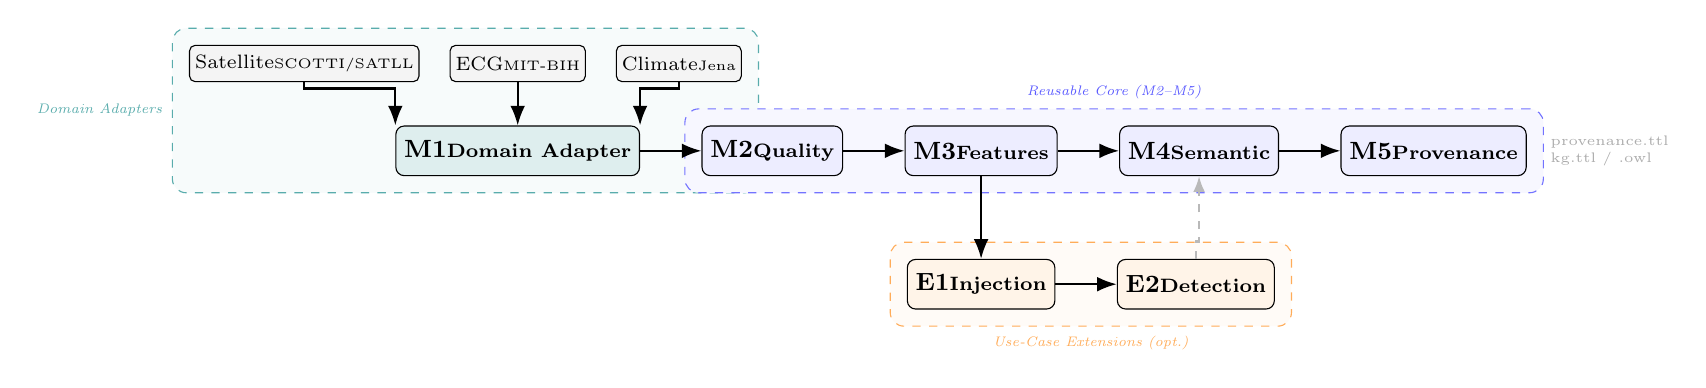
\begin{tikzpicture}[
  box/.style={draw, rounded corners=3pt, minimum width=1.65cm, minimum height=0.63cm,
              text centered, font=\small\bfseries, fill=white, inner sep=3pt},
  src/.style={draw, rounded corners=2pt, minimum width=1.25cm, minimum height=0.46cm,
              text centered, font=\scriptsize, fill=gray!9, inner sep=2pt},
  ext/.style={draw, rounded corners=3pt, minimum width=1.65cm, minimum height=0.63cm,
              text centered, font=\small\bfseries, fill=orange!9, inner sep=3pt},
  arr/.style={-{Latex[length=2.5mm]}, thick},
  darr/.style={-{Latex[length=2mm]}, thick, dashed, gray!55},
  node distance=0.5cm and 0.78cm
]
%% Data sources (top row)
\node[src] (dsrc1) {Satellite\\\tiny SCOTTI/SATLL};
\node[src, right=0.38cm of dsrc1] (dsrc2) {ECG\\\tiny MIT-BIH};
\node[src, right=0.38cm of dsrc2] (dsrc3) {Climate\\\tiny Jena};

%% M1 domain adapter (below sources, centred)
\node[box, below=0.55cm of dsrc2, fill=teal!13] (nm1)
  {M1\\\scriptsize Domain Adapter};
\draw[arr] (dsrc1.south) -- ++(0,-0.08) -| (nm1.north west);
\draw[arr] (dsrc2.south) -- (nm1.north);
\draw[arr] (dsrc3.south) -- ++(0,-0.08) -| (nm1.north east);

%% Core processing modules (horizontal chain right of M1)
\node[box, right=0.78cm of nm1, fill=blue!7] (nm2) {M2\\\scriptsize Quality};
\node[box, right=0.78cm of nm2, fill=blue!7] (nm3) {M3\\\scriptsize Features};
\node[box, right=0.78cm of nm3, fill=blue!7] (nm4) {M4\\\scriptsize Semantic};
\node[box, right=0.78cm of nm4, fill=blue!7] (nm5) {M5\\\scriptsize Provenance};

\draw[arr] (nm1) -- (nm2);
\draw[arr] (nm2) -- (nm3);
\draw[arr] (nm3) -- (nm4);
\draw[arr] (nm4) -- (nm5);

%% Use-case extensions (below M3 and M4)
\node[ext, below=1.05cm of nm3] (ne1) {E1\\\scriptsize Injection};
\node[ext, right=0.78cm of ne1] (ne2) {E2\\\scriptsize Detection};

\draw[arr] (nm3.south) -- ++(0,-0.26) -- (ne1.north);
\draw[arr] (ne1) -- (ne2);
\draw[darr] (ne2.north) -- ++(0,0.22) -| (nm4.south);

%% Output artifact label
\node[font=\tiny, right=0.18cm of nm5, align=left, text=gray!65]
  {provenance.ttl\\kg.ttl / .owl};

%% Background region annotations
\begin{scope}[on background layer]
  \node[draw=teal!65, dashed, rounded corners=5pt, fill=teal!3, inner sep=6pt,
        fit={(dsrc1)(dsrc2)(dsrc3)(nm1)},
        label={[font=\tiny\itshape,text=teal!65]left:Domain Adapters}] {};
  \node[draw=blue!55, dashed, rounded corners=5pt, fill=blue!3, inner sep=6pt,
        fit={(nm2)(nm3)(nm4)(nm5)},
        label={[font=\tiny\itshape,text=blue!65]above:Reusable Core (M2--M5)}] {};
  \node[draw=orange!65, dashed, rounded corners=5pt, fill=orange!3, inner sep=6pt,
        fit={(ne1)(ne2)},
        label={[font=\tiny\itshape,text=orange!65]below:Use-Case Extensions (opt.)}] {};
\end{scope}
\end{tikzpicture}
\caption{SensorWF architecture. The domain adapter (teal, M1) normalises raw sensor archives from three domains into a standardised DataFrame. The reusable core (blue, M2--M5) performs quality assessment, feature engineering, semantic annotation, and provenance export identically across all domains. Optional use-case extensions (orange, E1--E2) inject synthetic faults and evaluate ML detectors; E2 results optionally enhance M4's knowledge graph (dashed arrow). Switching domains requires only a new M1 adapter ($\approx$150\,lines of Python); M2--M5 require no modification.}
\label{fig:architecture}
\end{figure*}

\subsection{Design Principles}

The design of SensorWF is guided by five key principles.

\textbf{Core/extension separation.} The framework enforces a strict architectural boundary between a reusable core (M1--M5) and optional use-case extensions. The core is responsible for ingestion, quality assessment, feature engineering, semantic annotation, and provenance export, applied uniformly across all domains. Extensions, including fault injection (E1) and anomaly detection (E2), consume core typed outputs without modifying any core module. This separation is explicitly specified in \texttt{components.json} using an \texttt{extension} flag.

\textbf{Adapter isolation.} All domain-specific logic is encapsulated within M1 using the \texttt{DomainAdapter} abstract interface. Each adapter implements four methods: \texttt{load()}, \texttt{get\_quality\_config()}, \texttt{get\_feature\_config()}, and \texttt{get\_ontology\_path()}, which together provide comprehensive configuration for all downstream core modules. To support a new domain, only a new M1 adapter class (approximately 150 lines) must be implemented. Use-case extensions may also query \texttt{get\_fault\_types()}.

\textbf{Explicit I/O contracts.} Each module defines typed input and output ports that adhere to the ProvONE \texttt{provone:Program}/\texttt{provone:InPort}/\texttt{provone:OutPort} pattern \cite{missier2013provone}. These contracts are registered in \texttt{components.json} to facilitate programmatic discovery and composition.

\textbf{Scientific assumption transparency.} Domain assumptions, including sampling rates, quality thresholds, and window sizes, are recorded as \texttt{sensorwf:hasAssumption} predicates in both the static workflow specification and the runtime provenance trace. This method ensures that assumptions are directly SPARQL-queryable and remain auditable long after execution.

\textbf{Reproducibility by design.} All sources of randomness are controlled through a single seeded generator chain (\texttt{seed = 42}). Consequently, re-executing any domain entry point with the same seed produces bit-identical clean data, quality reports, feature matrices, and knowledge graph artifacts. Result caching---keyed on sentinel files (\texttt{run\_summary.json}, \texttt{ml\_results.csv})---avoids redundant recomputation, and the \texttt{--rerun} flag bypasses all caches to force a complete fresh execution.

\subsection{Component Registry and Module Descriptions}

\begin{table}[t]
\caption{SensorWF Component Registry -- Module Summary}
\label{tab:registry}
\centering
\scriptsize
\setlength{\tabcolsep}{3pt}
\begin{tabular}{@{}lp{1.7cm}p{4.1cm}@{}}
\toprule
\textbf{ID} & \textbf{Module} & \textbf{Key Assumptions / Contracts} \\
\midrule
\multicolumn{3}{l}{\textit{Core framework modules (M1--M5; all domains)}} \\
M1 & Data Ingestion     & Adapter-specified format; mandatory: \texttt{timestamp}, \texttt{elapsed\_s} \\
M2 & Quality Assessment & Stuck $\le k$ unique (adapter config); gap mult.\ 3--10$\times$ \\
M3 & Feature Engineering& 9 families/channel; Cython O($n$) skew/kurt; batched FFT \\
M4 & Semantic Annotation& SSN/SOSA-aligned OWL; feature-name--to--class lexical mapping \\
M5 & Provenance Export  & PROV-O/ProvONE Turtle; SHA-256 checksums; UTC ISO\,8601 \\
\midrule
\multicolumn{3}{l}{\textit{Use-case extensions (E1--E2; anomaly detection demonstration only)}} \\
E1 & Fault Injection    & 6--18 morphologies; amplitude $\times$ duration $\times$ spread tiers \\
E2 & Anomaly Detection  & Train on 60\% clean prefix; EVT/99th-pct.\ threshold; 5 detectors \\
\bottomrule
\end{tabular}
\end{table}

\textbf{M1: Data Ingestion.} Three adapters are implemented: \texttt{SatelliteAdapter} (SCOTTI v2 hex-encoded telemetry at approximately 1 Hz), \texttt{ECGAdapter} (MIT-BIH CSV at 360 Hz, decimated sevenfold to 50 Hz using a Chebyshev anti-alias filter, with 5-minute sessions yielding 15,000 samples), and \texttt{ClimateAdapter} (Jena CSV at 10-minute resolution, 14 channels, half-year slices). Each adapter returns a standardized DataFrame containing the mandatory columns \texttt{timestamp} and \texttt{elapsed\_s}, along with at least one signal channel.
\Logan{Expand}

\textbf{M2: Quality Assessment.} Quality checks are determined by the adapter's \texttt{get\_quality\_config()} dictionary, ensuring that M2 remains domain-agnostic. The module evaluates NaN rates, stuck-sensor patterns (defined as $\le k$ unique values within a window), timing regularity (exceeding $n$ times the expected sample interval), per-channel Z-score outliers, and optional linear-trend artifacts. The outputs include a quality report in JSON format and a cleaned DataFrame.

\textbf{M3: Feature Engineering.} Nine feature families are constructed per channel when session length is at least $3\times$ the rolling window: (i)~raw channel value; (ii)~first-order difference; (iii)~rolling mean; (iv)~rolling standard deviation; (v)~rolling skewness; (vi)~rolling excess kurtosis; (vii)~zero-crossing rate relative to the channel mean; (viii)~spectral entropy (Shannon entropy of the rolling power spectrum, computed via vectorised batched FFT); and (ix)~dominant frequency in Hz (peak non-DC frequency). Rolling skewness and kurtosis are computed by a Cython-compiled O($n$) sliding-window accumulator (\texttt{scripts/\_core\_cy.pyx}, \texttt{-O3 -ffast-math}), and spectral features use a 3-D stride-tricks FFT across all channels simultaneously. A timing feature (\texttt{dt\_sample}) derived from \texttt{elapsed\_s} is always appended. The resulting feature matrix has dimensions $N \times D$, where $D$ is determined by the channel count and window size.

\textbf{M4: Semantic Annotation.} Feature importances are mapped to a domain-specific OWL ontology using lexical prefix matching on feature names. The resulting knowledge graph includes OWL class-instance nodes, feature nodes, and evidence edges with the \texttt{if:featureImportance} and \texttt{if:evidenceForClass} predicates, supporting SPARQL-queryable subsystem attribution. When executed after E2, anomaly tag nodes are incorporated; in core-only mode, edges represent feature-to-class evidence derived directly from the M3 feature matrix. Outputs include RDF/Turtle and CSV node and edge lists.

\textbf{M5: Provenance Export.} The \texttt{ProvenanceRecorder} records one \texttt{prov:Activity} for each module invocation, capturing wall-clock timestamps, input row counts, output file paths, and parameter values. SHA-256 checksums are computed automatically for all file-path entities and stored as \texttt{telwf:sha256} triples, enabling bit-level reproducibility verification. The serialized PROV-O/ProvONE Turtle document serves as the primary workflow output and is generated regardless of whether the use-case extension is executed.

\textbf{E1: Fault Injection (use-case only).} The module reads \texttt{get\_fault\_types()} and applies each morphology across three difficulty tiers, scaling amplitude, duration, and channel spread simultaneously. This multi-axis approach mitigates the confounds of single-axis separability described by Wu and Keogh \cite{wu2022benchmarks}. With two variants per (type, tier) pair, E1 generates $N_{\text{faults}} \times 3 \times 2$ labeled sessions per domain (see Table~\ref{tab:m4params}).

\textbf{E2: Anomaly Detection (use-case only).} Five machine learning detectors are trained on the first 60\% of the clean session (prior to any injected segment): (i)~Z-Score with MAD-robust fusion (Iglewicz-Hoaglin threshold \cite{iglewicz1993outliers}); (ii)~RobustRollingZScore with CUSUM persistence \cite{page1954cusum}; (iii)~IsolationForest with a three-member contiguous-feature rotation ensemble \cite{liu2008isolation}; (iv)~a multi-scale MLP Autoencoder with Gaussian denoising ($\sigma=0.06$), dual sequence windows (lengths 8 and 16), and two hidden layers (64 and 32 units, tanh activations) \cite{sakurada2014autoencoder}; and (v)~Local Outlier Factor (LOF) with novelty detection and PCA pre-processing (95\% variance retained) \cite{breunig2000lof}. Ensemble and density-based detectors (IF, LOF, PCA) use scikit-learn \cite{pedregosa2011sklearn}. For density-based detectors (IF and LOF), Peaks-over-Threshold (POT) EVT calibration \cite{siffer2017evt} fits a Generalized Pareto Distribution to the tails of the training-set scores, whereas statistical detectors use the 99th percentile threshold. Per-fault and aggregate metrics, including AUC-ROC, AUC-PR, F1, FPR, recall, and the binary \texttt{event\_detected} metric, are reported by tier.

\subsection{Domain Applications}

\subsubsection{Satellite Telemetry (KISPE SATLL)}

The KISPE Satellite Learning Laboratory (SATLL) provides authentic telemetry from four experiment families: AccelerometerTest, GyroTest, ReactionWheelTest, and ThermalTest \cite{kispe_satll}. Each session generates CDH (Command and Data Handling) data, encompassing 87 columns including measurements of thermal, power, and timing, as well as ADCS (Attitude Determination and Control System) data, covering 30 columns that include sensors for inertia measurement units (IMUs), reaction wheels, and sun sensors, at approximately 1 Hz. E1 introduces 18 fault types: 16 single-channel faults and 2 compound faults involving multiple channels. CDH faults encompass issues such as power-rail drift, thermal ramp, and packet dropout, while ADCS faults include gyro clipping, magnetometer inversion, and wheel runaway or stiction. For each experiment family, there are 108 labeled sessions ($18 \times 3 \times 2 = 108$).

The satellite OWL ontology is generated by the pipeline at runtime. The script \texttt{satellite\_ontology.py} examines the CDH and ADCS channel lists identified during M1 and produces an OWL/XML document containing subsystem classes (\texttt{sat:ADCS}, \texttt{sat:OBDH}, \texttt{sat:EPS}, \texttt{sat:ThermalControlSubsystem}), sensor-type subclasses, and individual channels. Alignment with SSN and SOSA is achieved through the use of \texttt{sosa:Platform} and \texttt{ssn:Sensor} superclasses. The combined single-session M4 run across 122 channels produces 1,104 knowledge graph nodes and 846 edges.

\subsubsection{Biomedical ECG (MIT-BIH Arrhythmia Database)}

The MIT-BIH Arrhythmia Database \cite{moody2001mitbih} comprises 48 thirty-minute, two-lead ambulatory ECG recordings at 360 Hz from PhysioNet \cite{goldberger2000physiobank}, each annotated beat-by-beat by cardiologists. Twenty records are selected to represent all major rhythm classes: normal sinus rhythm (100, 101, 103, 112, 113, 115), bundle branch block (106, 108, 109, 111, 118), frequent premature ventricular contractions (PVCs) and bigeminy (105, 119, 200, 205, 215), and atrial fibrillation with complex ventricular rhythms (201, 208, 213, 221). The \texttt{ECGAdapter} applies a Chebyshev Type I low-pass filter (cut-off 22 Hz, order 4) prior to decimation by a factor of 7 to 50 Hz, thereby preventing aliasing above the Nyquist limit of 25 Hz. Six ECG-specific fault morphologies are introduced: baseline wander, electrode dropout, EMG burst, powerline noise (10 Hz, representing the alias of 60 Hz mains interference after decimation: $60 \bmod 50 = 10$ Hz), amplitude scaling, and lead inversion. For each record, $6 \times 3 \times 2 = 36$ labeled sessions are generated.

\subsubsection{Atmospheric Climate (Jena Climate Dataset)}

The Jena Climate Dataset \cite{jena_climate} records 14 meteorological variables, including temperature, pressure, humidity, and wind speed or direction, at 10-minute intervals from 2009 to 2016 (420,551 rows). The \texttt{ClimateAdapter} extracts half-year segments (approximately 26,000 rows each) and removes $-9999$ sentinel values. M3 employs a 24-sample rolling window (4 hours). Seven half-year sessions from 2009 to 2015 are processed, collectively covering cold and warm seasons, distinct instrument drift periods, and seven years of inter-annual variability. Six climate-specific fault morphologies are introduced: sensor drift, stuck sensor, spike burst, sensor dropout, scale error, and sign flip. For each session, $6 \times 3 \times 2 = 36$ labeled sessions are produced.

%% =========================================================
\section{Domain Application Results}
\label{sec:results}
%% =========================================================

\begin{table}[t]
\caption{Cross-Domain Detection Performance (All Tiers, Session-Averaged)}
\label{tab:crossdomain}
\centering
\scriptsize
\setlength{\tabcolsep}{2.5pt}
\begin{tabular}{@{}lrrccccc@{}}
\toprule
 & & & \multicolumn{5}{c}{\textbf{AUC-ROC / AUC-PR}} \\
\cmidrule(lr){4-8}
\textbf{Domain} & \textbf{Sess.} & \textbf{Faults} & \textbf{AE} & \textbf{IF} & \textbf{LOF} & \textbf{RRZS} & \textbf{ZS} \\
\midrule
Satellite (SATLL) & 1  & 18 & \textbf{0.772}/\textbf{0.581} & 0.564/0.298 & 0.549/0.280 & 0.597/0.359 & 0.610/0.394 \\
ECG (MIT-BIH)     & 20 &  6 & 0.915/0.837 & 0.880/0.762 & \textbf{0.918}/\textbf{0.826} & 0.487/0.394 & 0.785/0.637 \\
Climate (Jena)    &  7 &  6 & \textbf{0.835}/\textbf{0.725} & 0.720/0.577 & 0.737/0.609 & 0.536/0.399 & 0.681/0.552 \\
\bottomrule
\multicolumn{8}{l}{\scriptsize AE=Autoencoder, IF=IsolationForest, LOF=Local Outlier Factor,} \\
\multicolumn{8}{l}{\scriptsize RRZS=RobustRollingZScore, ZS=ZScore. Bold: best per domain.} \\
\multicolumn{8}{l}{\scriptsize ECG std: AE $\pm$0.055, LOF $\pm$0.042; Climate: AE $\pm$0.023, LOF $\pm$0.041.}
\end{tabular}
\end{table}

\begin{figure}[t]
\centering
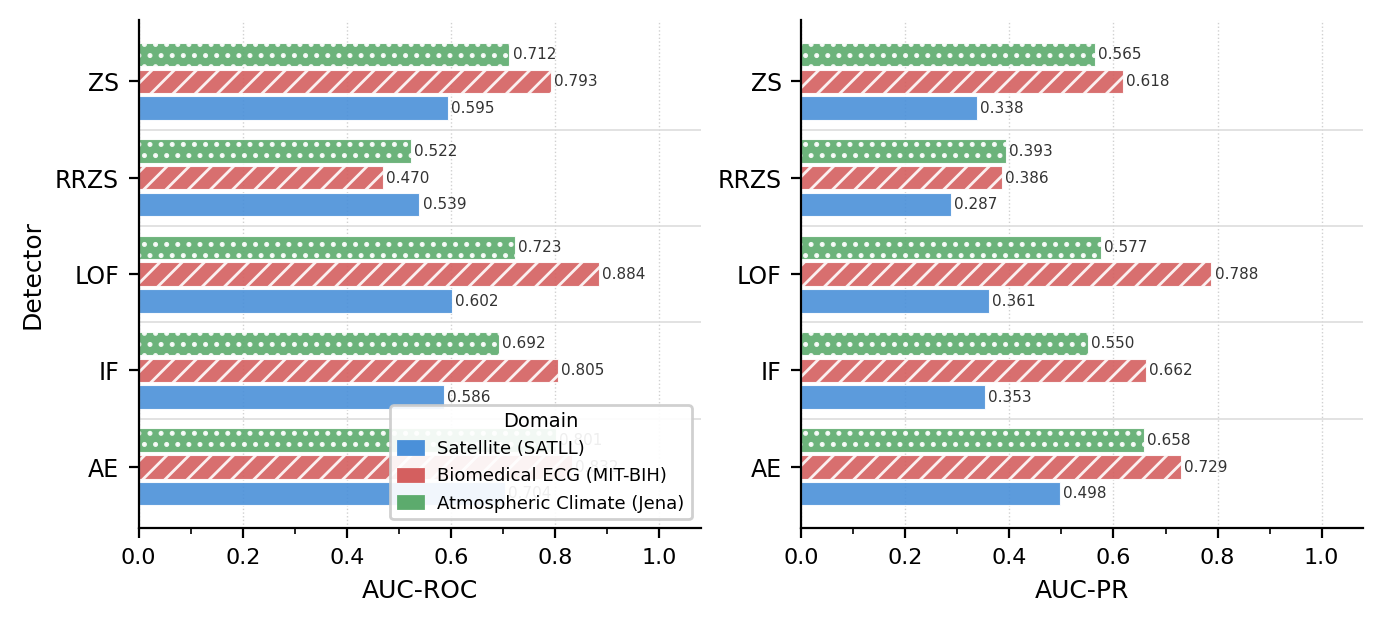
\includegraphics[width=\columnwidth]{figures/fig_domain_comparison.png}
\caption{Cross-domain detection performance for all five E2 detectors across satellite (SATLL), biomedical ECG (MIT-BIH), and atmospheric climate (Jena). Values are macro-averaged over all sessions per domain. AE=Autoencoder, IF=IsolationForest, RRZS=RobustRollingZScore, ZS=ZScore.}
\label{fig:crossdomain}
\end{figure}

\subsection{Training and Evaluation Protocol}
\label{sec:protocol}

E2 enforces a strict temporal train/test split to prevent leakage. The first 60\% of each clean baseline session serves as training data. E1 targets only the held-out 40\% suffix: injected windows always begin at or after sample $\lfloor 0.6 \cdot N \rfloor$, ensuring zero temporal overlap between the training prefix and any evaluated anomalous segment. Rolling-window features (maximum 100 samples at 50 Hz) are negligibly small relative to the $\geq\!6{,}000$-sample clean gap, preventing roll-back leakage. Evaluation reports sample-wise AUC-ROC, AUC-PR, F1, FPR, recall, and \texttt{event\_detected} (binary: was the injected anomaly window intercepted by at least one true positive?), averaged over all injection variants and grouped by difficulty tier. AUC-PR is the primary imbalance-aware metric given anomaly prevalence of $\approx\!20$--$40\%$ per injected session. Table~\ref{tab:m4params} gives exact E1 parameter ranges across all three domains and difficulty tiers.

\begin{table}[t]
\caption{E1 Fault Injection -- Parameter Ranges by Difficulty Tier}
\label{tab:m4params}
\centering
\scriptsize
\setlength{\tabcolsep}{3pt}
\begin{tabular}{@{}lcccc@{}}
\toprule
\textbf{Tier} & \textbf{Amp.\ scale} & \textbf{Dur.\ frac.\ of $N$} & \textbf{Ch.\ spread} & \textbf{Difficulty} \\
\midrule
Easy   & $1.45\times\sigma$ & $0.30$ & $1.25\times$ & Low \\
Medium & $1.05\times\sigma$ & $0.95$ & $1.00\times$ & Medium \\
Hard   & $0.72\times\sigma$ & $1.55$ & $0.70\times$ & High \\
\bottomrule
\end{tabular}
{\vspace{2pt}\scriptsize Amplitude scale: peak anomaly deviation as multiple of per-channel signal $\sigma$. Duration fraction: multiplier on a nominal window of $0.40 \cdot N$. Channel spread: multiplier on reference channel count (compound faults only). Parameters are domain-invariant; applied identically for satellite, ECG, and climate. Absolute session lengths: satellite $\approx\!1800$\,s; ECG 15,000 samples @ 50\,Hz; climate 26,280 samples @ 6/hr.}
\end{table}

\subsection{Satellite Telemetry (KISPE SATLL)}

On the satellite domain, the Autoencoder leads all five detectors with AUC-ROC $0.772$ and AUC-PR $0.581$, consistent with its temporal reconstruction capacity for the multi-channel CDH and ADCS fault morphologies. Notably, the detector ranking for satellite differs substantially from the ECG and Climate domains: ZScore ranks second (AUC-ROC $0.610$, AUC-PR $0.394$) and RobustRollingZScore third ($0.597$/$0.359$), while IsolationForest ($0.564$/$0.298$) and LOF ($0.549$/$0.280$) rank last. This reversal of the density-based detectors is attributable to the short session length (333 rows), which limits the training prefix to $\approx\!200$ samples---insufficient for LOF and IsolationForest to build reliable density estimates across 122 channels. The Autoencoder's reconstruction loss is less sensitive to training-set size in low-row settings, making it the most robust choice for this domain. Easy-tier faults yield the highest Autoencoder AUC-ROC ($0.801$) due to the larger amplitude injections, while Hard-tier produces the highest AUC-PR ($0.646$) as the longer fractional window increases the positive class rate.

\subsection{Biomedical ECG (MIT-BIH Arrhythmia Database)}

On the ECG domain, LOF achieves the highest AUC-ROC ($0.918 \pm 0.042$) and AUC-PR ($0.826 \pm 0.088$) across all 20 records, narrowly outperforming the Autoencoder (AUC-ROC $0.915 \pm 0.055$, AUC-PR $0.837 \pm 0.097$) and IsolationForest ($0.880$/$0.762$). The two leading detectors are effectively tied on AUC-ROC, but the Autoencoder marginally leads on AUC-PR ($0.837$ vs.\ $0.826$), reflecting its advantage on harder-tier faults where the longer injected windows raise the precision-recall operating point. Six morphologically distinct fault types produce compact, well-separated clusters in the 19-feature rolling-window space, favouring both neighbourhood-density estimation and reconstruction-based approaches. Low standard deviations for IF ($\pm 0.047$) and LOF ($\pm 0.042$) confirm stability across the 20-record rhythm-class mix. RobustRollingZScore performs poorly (AUC-ROC $0.487$, AUC-PR $0.394$), consistent with its fixed-window assumption breaking down against the varied morphologies of ECG artefact injections. Per-tier results show strong performance across all difficulty levels for AE and LOF, with AUC-ROC ranging from $0.876$ (Hard) to $0.943$ (Easy) and $0.886$ (Hard) to $0.947$ (Easy) respectively; full per-tier numeric results are given in Appendix~\ref{app:tier}.

\subsection{Atmospheric Climate (Jena Climate Dataset)}

On the climate domain, the Autoencoder leads with AUC-ROC $0.835$ and AUC-PR $0.725$, with notably low variance across the seven half-year sessions ($\pm 0.023$), confirming consistent detection of sustained meteorological sensor faults across seven years of seasonal and inter-annual variability. LOF ranks second (AUC-ROC $0.737 \pm 0.041$, AUC-PR $0.609 \pm 0.055$), and IsolationForest third ($0.720$/$0.577$). ZScore ($0.681$/$0.552$) outperforms RobustRollingZScore ($0.536$/$0.399$); the RRZS degradation on climate faults is consistent with its sensitivity to variable anomaly duration across tiers. The Hard-tier AUC-PR values substantially exceed Easy-tier for all detectors (e.g., AE: $0.856$ vs.\ $0.549$), driven by the larger fractional window occupied by Hard-tier injections increasing the positive class rate. IsolationForest shows the largest gap between AUC-ROC and AUC-PR ($0.720$ vs.\ $0.577$ overall), indicating weaker calibration at the precision-recall operating point for climate fault distributions.

\subsection{Semantic Knowledge Graph}

The satellite core M4 run produces a knowledge graph with 1,104 nodes and 846 edges; after E2, the ML-enhanced KG incorporates IsolationForest feature importances, producing 23 ML-weighted nodes linked to subsystem classes. The top SPARQL-queried evidence class is \texttt{sat:AttitudeDeterminationAndControlSubsystem}, consistent with the ADCS-heavy channel structure. Fig.~\ref{fig:kgsubgraph} illustrates the resulting subgraph. The \texttt{if:featureImportance} predicate supports queries of the form \texttt{SELECT ?feat ?cls WHERE \{?feat if:evidenceForClass ?cls\}} without rerunning the detector, enabling post-hoc subsystem attribution; channel-level attribution methods \cite{condattrib2026,multiviewae2026} are identified as a complementary extension for explaining individual anomaly scores at the channel and time-step level. For ECG, per-record M4 runs produce compact knowledge graphs averaging 20 nodes and 9 edges each (401 nodes and 189 edges total across 20 records), reflecting the two-channel signal structure (19 features per record). For Climate, per-session M4 runs produce substantially larger graphs (987 total nodes and 882 total edges across 7 sessions) due to the 127 features derived from 14 meteorological channels.

\begin{figure}[t]
\centering
\includegraphics[width=\columnwidth]{figures/fig_kg_subgraph.png}
\caption{M4 knowledge graph subgraph for the satellite domain (AccelerometerTest family). Nodes represent OWL class instances (\texttt{sat:ADCS}, \texttt{sat:OBDH}, etc.), anomaly tags, and IsolationForest feature nodes. Edges carry \texttt{if:featureImportance} and \texttt{if:evidenceForClass} predicates, enabling SPARQL queries that link detector evidence to satellite engineering subsystems without re-executing the detector.}
\label{fig:kgsubgraph}
\end{figure}

\subsection{Runtime Characterisation}

Table~\ref{tab:runtime} gives per-module wall-clock times measured on a standard laptop (Apple M-series, single thread). E2 accounts for roughly 80--90\% of total pipeline time; a detector-fit cache---keyed on detector configuration rather than fault tag---ensures each family incurs exactly one training pass and re-evaluates all $N_{\text{faults}} \times 3 \times 2$ variants without redundant model refits. Correcting a prior defect that re-trained all five detectors once per fault tag ($6\times$ redundant Autoencoder fits per record) reduced ECG E2 time from $>\!1{,}000$\,s per record to the values shown. Core modules M1--M5 together consume less than 10\% of runtime, confirming that framework overhead is negligible relative to domain analysis costs. M3 remains under 1\,s across all domains thanks to the Cython-compiled skew/kurtosis accumulator and the batched stride-tricks FFT.

\begin{table}[t]
\caption{Per-Module Runtime (Satellite, 4 Families, 2 Variants, 3 Tiers)}
\label{tab:runtime}
\centering
\scriptsize
\setlength{\tabcolsep}{3.5pt}
\begin{tabular}{@{}lrrl@{}}
\toprule
\textbf{Module} & \textbf{Time (s)} & \textbf{\%} & \textbf{Notes} \\
\midrule
M1 Ingestion     & $<$1     & $<$1  & Parse SCOTTI archive \\
M2 Quality       & $<$1     & $<$1  & Clean + flag channels \\
M3 Features      & $<$1     & $<$1  & 9 families; Cython O($n$) + batched FFT \\
E1 Injection     & $\sim$5  & $\sim$1  & Generate 432 labelled CSVs \\
E2 Detection     & $\sim$400 & $\sim$90 & Train 5 ML detectors; config-keyed cache \\
M4 Semantic      & $\sim$30 & $\sim$7  & Build KG from ML evidence + OWL \\
M5 Provenance    & $<$1     & $<$1  & Serialise PROV-O trace + SHA-256 \\
\midrule
Total            & $\sim$440 & 100  & Single laptop, no GPU \\
\bottomrule
\end{tabular}
\end{table}

\Logan{Better way to word this section? ``Use-Case Results''? This is where we discuss the performance of our workflow when applied}

%% =========================================================
\section{Discussion}
\label{sec:discussion}
%% =========================================================

\subsection{Generalizability and Adapter Effort}

For the three validated domains, implementing each adapter required approximately 150--200 lines of Python; M2--M5 required no code modifications. The component registry enables programmatic composition: a consumer queries \texttt{components.json} for modules with a given \texttt{domain\_tag} and receives fully specified I/O contracts, enabling automated workflow instantiation and validation. The claim that \emph{only M1 is domain-specific} holds at the code level but warrants a practical qualification: M2--M5 behaviour depends on adapter-supplied configuration dictionaries that themselves encode domain knowledge the adapter author must provide explicitly. Portability limitations---e.g., M2 assumes temporally regular sampling; irregular-rate or event-driven streams require time-indexed rolling windows in M3 and resampling extensions in M2---are documented as \texttt{sensorwf:hasAssumption} predicates in the registry.

\subsection{FAIR Assessment}

Table~\ref{tab:fair} assesses SensorWF against the four FAIR dimensions. Reproducibility is guaranteed at the code level: running any domain entry point with \texttt{--seed 42} produces bit-identical CSVs, injection summaries, metrics, and KG artefacts. The only run-variant output is \texttt{provenance.ttl}, whose timestamps differ by design. Workflow registration on WorkflowHub with RO-Crate metadata and immutable Zenodo archives are planned for the open scientific object release.

\begin{table}[t]
\caption{SensorWF FAIR Assessment}
\label{tab:fair}
\centering
\scriptsize
\setlength{\tabcolsep}{3pt}
\begin{tabular}{@{}lp{5.4cm}@{}}
\toprule
\textbf{Principle} & \textbf{SensorWF Implementation} \\
\midrule
\textbf{Findable}      & \texttt{components.json} registry; SHA-256-checksummed provenance published with code; DOI via Zenodo (planned) \\
\textbf{Accessible}    & Open formats: CSV, JSON, RDF/Turtle, OWL; three public benchmark datasets; self-contained per-domain HTML run report (quality tables, aggregated ML results, embedded figures, live KG visualisation) \\
\textbf{Interoperable} & PROV-O + ProvONE; SSN/SOSA-aligned OWL; standardised DataFrame schema; typed module contracts \\
\textbf{Reusable}      & Domain assumptions encoded in machine-readable component registry; any sensor domain can be integrated without altering the analytical core; \texttt{DomainAdapter} interface; seeded RNG; \texttt{--rerun} cache bypass; \texttt{sensorwf:hasAssumption} predicates \\
\bottomrule
\end{tabular}
\end{table}

\subsection{Relation to Satellite Anomaly Benchmarks}

The ESA-ADB benchmark \cite{esa_adb2024} recommends event-level ground truth, affiliation-aware scoring, and dynamic/EVT thresholding with postprocessing for operational satellite telemetry. OPS-SAT \cite{ruszczak2025opssat} emphasises segment-level precision at low operating FPR. SensorWF partially addresses these recommendations: density-based detectors (IF, LOF) use POT EVT calibration (Section~\ref{sec:protocol}), and an event-level \texttt{event\_detected} metric is emitted per variant. Full affiliation-aware scoring and dynamic postprocessing remain priority extensions. E2's threshold strategy and detector suite are registry-declared parameters, facilitating incremental alignment with ESA-ADB protocols without modifying any core module.

%% =========================================================
\section{Limitations and Future Work}
\label{sec:limitations}
%% =========================================================

\textbf{Synthetic-only evaluation.} All ground-truth labels are generated by E1; no real annotated anomalies are used. This risks overstating generality relative to operational benchmark performance (e.g., ESA-ADB, OPS-SAT). Evaluation on real annotated datasets is a priority extension.

\textbf{Sample-wise metrics.} AUC-ROC and AUC-PR are computed at the sample level; the binary \texttt{event\_detected} flag adds an event-level complement per variant. Event-wise, affiliation-aware, and range-based metrics \cite{esa_adb2024,lavin2015nab} better reflect detection quality for operational use and are identified as a priority extension.

\textbf{Deep learning baselines.} The five E2 detectors do not include LSTM-based encoder-decoder models \cite{malhotra2016lstm}, transformer-based approaches such as Anomaly Transformer \cite{xu2022anomalytransformer} or TranAD \cite{tuli2022tranad}, or robust variational autoencoder variants \cite{rvaest2025,streamvae2025}, all of which require separate deep learning frameworks. The registry-based E2 architecture accommodates these; integrating at least one transformer baseline is planned as the immediate next step. Adaptive multi-detector selection strategies \cite{ramses2026} represent a further extension toward runtime ensemble composition within the E2 registry.

\textbf{Provenance completeness.} SHA-256 checksums are computed automatically for all file-path entities and stored as \texttt{telwf:sha256} triples, enabling bit-level reproducibility verification. Ontology class mappings have not been externally validated by domain experts; the current lexical prefix-matching heuristic is a practical approximation pending expert review.

%% =========================================================
\section{Conclusion}
\label{sec:conclusion}
%% =========================================================

SensorWF demonstrates that a FAIR-annotated, generalizable workflow framework for scientific sensor time-series analysis is both tractable and practically useful across disciplinary boundaries. Separating domain-specific ingestion (M1 adapter) from a reusable analytical core (M2--M5) and encoding domain assumptions in a machine-readable component registry---so that any sensor domain can be integrated and reused without altering the analytical core---lets researchers adopt, adapt, and extend a common pipeline without per-domain reimplementation. Use-case extensions (E1 fault injection, E2 anomaly detection) attach to core typed outputs without modifying any core module, demonstrating that the architecture supports diverse downstream analyses.

Cross-domain validation across spacecraft telemetry (KISPE SATLL, 1 session, 18 fault types), ambulatory ECG (20 MIT-BIH records spanning all major rhythm classes), and atmospheric climate (7 Jena half-year sessions) shows that a consistent detection architecture emerges from a single codebase with domain-specific configuration exclusively in M1. On satellite, the Autoencoder leads (AUC-ROC $0.772$, AUC-PR $0.581$), with density-based detectors ranking last due to the short session constraining the training prefix to $\approx$200 samples. On ECG, LOF and the Autoencoder are effectively tied for best performance (AUC-ROC $0.918\pm0.042$ and $0.915\pm0.055$, AUC-PR $0.826$ and $0.837$ respectively), with the Autoencoder narrowly leading on AUC-PR. On climate, the Autoencoder leads (AUC-ROC $0.835\pm0.023$, AUC-PR $0.725$) with notably low variance across seven years of sessions. EVT-calibrated thresholding for density-based detectors, rolling-window sensitivity analysis, and an event-level detection metric strengthen the evaluation protocol. Key remaining limitations---synthetic-only evaluation, point-wise metrics, and the absence of transformer baselines---are explicitly documented as \texttt{sensorwf:hasAssumption} predicates. KISPE SATLL data and all code will be released on GitHub as an open scientific object.

%% =========================================================
\section*{Acknowledgment}
%% =========================================================

\Alex{Joe: Please thank the person from KISPE who helped us to retrieve the data from the satellite.}
\Alex{Kellan: Thank CARS, money from them, I'll send you the text with grant number, the ERAU CoE for providing the satellite.}
The authors thank KISPE Space Systems for access to the SATLL telemetry datasets, PhysioNet for the MIT-BIH Arrhythmia Database, and the Max Planck Institute for Biogeochemistry for the Jena Climate Dataset.

%% =========================================================
\bibliographystyle{IEEEtran}
\bibliography{main}

%% =========================================================
\appendices
%% =========================================================

\section{ECG Detection Performance by Difficulty Tier}
\label{app:tier}

Table~\ref{tab:tier} disaggregates the ECG AUC-ROC and AUC-PR results (averaged across all 20 MIT-BIH records) by the three E1 difficulty tiers. AUC-PR increases monotonically from Easy to Hard for all detectors because Hard-tier injections occupy a larger fractional window, reducing effective class imbalance. AUC-ROC is highest on Easy for AE and LOF, reflecting their superior detection of the largest-amplitude faults; IF follows the same trend. RobustRollingZScore is near-random ($\approx\!0.49$) across all tiers, confirming its insensitivity to the varied ECG artefact morphologies.

\begin{table}[h]
\caption{ECG AUC-ROC / AUC-PR by Difficulty Tier (20 Records, 6 Fault Types)}
\label{tab:tier}
\centering
\scriptsize
\setlength{\tabcolsep}{2.5pt}
\begin{tabular}{@{}llrrrrr@{}}
\toprule
\textbf{Tier} & \textbf{Det.} & \textbf{AUC-ROC} & \textbf{AUC-PR} & \textbf{Recall} & \textbf{FPR} & \textbf{F1} \\
\midrule
Easy   & AE   & \textbf{0.943} & 0.762 & 0.806 & 0.072 & 0.674 \\
       & IF   & 0.906 & 0.638 & 0.552 & 0.037 & 0.517 \\
       & LOF  & \textbf{0.947} & 0.729 & 0.841 & 0.113 & 0.631 \\
       & RRZS & 0.482 & 0.153 & 0.055 & 0.028 & 0.075 \\
       & ZS   & 0.809 & 0.441 & 0.242 & 0.048 & 0.218 \\
\midrule
Medium & AE   & \textbf{0.927} & 0.861 & 0.768 & 0.087 & 0.753 \\
       & IF   & 0.889 & 0.793 & 0.496 & 0.044 & 0.514 \\
       & LOF  & \textbf{0.921} & 0.851 & 0.798 & 0.135 & 0.763 \\
       & RRZS & 0.483 & 0.399 & 0.059 & 0.028 & 0.094 \\
       & ZS   & 0.789 & 0.671 & 0.219 & 0.048 & 0.239 \\
\midrule
Hard   & AE   & 0.876 & \textbf{0.888} & 0.660 & 0.078 & 0.690 \\
       & IF   & 0.844 & 0.854 & 0.388 & 0.043 & 0.430 \\
       & LOF  & 0.886 & \textbf{0.899} & 0.701 & 0.097 & 0.742 \\
       & RRZS & 0.495 & 0.630 & 0.062 & 0.029 & 0.104 \\
       & ZS   & 0.757 & 0.799 & 0.160 & 0.043 & 0.202 \\
\bottomrule
\multicolumn{7}{l}{\scriptsize AE=Autoencoder, IF=IsolationForest, RRZS=RobustRollingZScore, ZS=ZScore.} \\
\multicolumn{7}{l}{\scriptsize Bold: best AUC-ROC and AUC-PR per tier. Averaged across 20 records, 6 fault types.}
\end{tabular}
\end{table}

\section{M4 Knowledge Graph SPARQL Query Examples}
\label{app:sparql}

The following queries illustrate the post-hoc analytical value of the M4 knowledge graph without re-executing any ML detector.

\noindent\textbf{Q1: Which satellite subsystems carry the strongest anomaly evidence?}
\begin{lstlisting}[basicstyle=\ttfamily\scriptsize]
PREFIX if: <http://sensorwf.org/interpretability#>
PREFIX sat: <http://sensorwf.org/satellite#>
SELECT ?subsystem (SUM(?imp) AS ?total_evidence)
WHERE {
  ?feat if:belongsToSubsystem ?subsystem ;
        if:featureImportance ?imp .
}
GROUP BY ?subsystem ORDER BY DESC(?total_evidence)
\end{lstlisting}

\noindent\textbf{Q2: Top-5 features by IsolationForest importance for gyro faults:}
\begin{lstlisting}[basicstyle=\ttfamily\scriptsize]
PREFIX if: <http://sensorwf.org/interpretability#>
SELECT ?feat ?cls ?imp
WHERE {
  if:tag:A2_gyro_clipping if:importantFeature ?feat .
  ?feat if:featureImportance ?imp ;
        if:mapsToSensorClass ?cls .
}
ORDER BY DESC(?imp) LIMIT 5
\end{lstlisting}

These queries execute against the RDF/Turtle graph (\texttt{if\_ontology\_graph.ttl}) produced by M4 using any SPARQL~1.1 endpoint (e.g., Apache Jena Fuseki, RDFLib). No Python or ML libraries are required for post-hoc subsystem attribution.

\section{M3 Rolling-Window Ablation -- Full Numeric Results}
\label{app:ablation}

Table~\ref{tab:ablation_full} gives the complete per-detector AUC-ROC and AUC-PR values underlying Fig.~\ref{fig:ablation}. Results are averaged over all fault types and three difficulty tiers for 5 MIT-BIH ECG records.

\begin{table}[h]
\caption{M3 Window Ablation -- Mean AUC-ROC / AUC-PR (ECG, 5 Records)}
\label{tab:ablation_full}
\centering
\scriptsize
\setlength{\tabcolsep}{3pt}
\begin{tabular}{@{}lrrrrr@{}}
\toprule
 & \multicolumn{5}{c}{\textbf{AUC-ROC (AUC-PR)}} \\
\cmidrule{2-6}
$w$ & \textbf{AE} & \textbf{IF} & \textbf{LOF} & \textbf{RRZS} & \textbf{ZS} \\
\midrule
  15 & 0.775 (0.651) & 0.707 (0.554) & 0.854 (0.768) & 0.449 (0.370) & 0.688 (0.523) \\
  30 & 0.797 (0.671) & 0.758 (0.594) & 0.869 (0.777) & 0.452 (0.371) & 0.756 (0.575) \\
  50 & 0.793 (0.671) & 0.803 (0.647) & 0.868 (0.773) & 0.462 (0.382) & 0.794 (0.612) \\
 100 & 0.807 (0.694) & 0.816 (0.671) & 0.876 (0.780) & 0.464 (0.388) & 0.806 (0.625) \\
\bottomrule
\end{tabular}
\end{table}

\end{document}
